%                                                                 aa.dem
% AA vers. 9.1, LaTeX class for Astronomy & Astrophysics
% demonstration file
%                                                       (c) EDP Sciences
%-----------------------------------------------------------------------
%
% \documentclass[referee]{aa} % for a referee version
%\documentclass[onecolumn]{aa} % for a paper on 1 column  
%\documentclass[longauth]{aa} % for the long lists of affiliations 
%\documentclass[letter]{aa} % for the letters 
%\documentclass[bibyear]{aa} % if the references are not structured 
%                              according to the author-year natbib style

%

\documentclass{aa}  

%
\usepackage{graphicx}
\usepackage{amsmath,amsfonts,amssymb}
\usepackage{natbib}


%%%%%%%%%%%%%%%%%%%%%%%%%%%%%%%%%%%%%%%%
\usepackage{txfonts}
\usepackage{xcolor}

\usepackage{blindtext}
%%%%%%%%%%%%%%%%%%%%%%%%%%%%%%%%%%%%%%%%
% \usepackage[options]{hyperref}
% To add links in your PDF file, use the package "hyperref"
% with options according to your LaTeX or PDFLaTeX drivers.
\usepackage{float}
%\usepackage{stfloats}
\usepackage{dblfloatfix}
\usepackage{afterpage}
\usepackage{ifthen}
\usepackage[morefloats=12]{morefloats}

\usepackage{placeins}
\usepackage{multicol}
\usepackage[export]{adjustbox}\usepackage[breaklinks,colorlinks,citecolor=blue]{hyperref}
\bibpunct{(}{)}{;}{a}{}{,}
\usepackage[switch]{lineno}
\definecolor{linkcolor}{rgb}{0.6,0,0}
\definecolor{citecolor}{rgb}{0,0,0.75}
\definecolor{urlcolor}{rgb}{0.12,0.46,0.7}
%\usepackage[breaklinks, colorlinks, urlcolor=urlcolor,linkcolor=linkcolor,citecolor=citecolor,pdfencoding=auto]{hyperref}
\hypersetup{linktocpage}
\usepackage{bold-extra}
\usepackage{tabularx, booktabs}



\def\setsymbol#1#2{\expandafter\def\csname #1\endcsname{#2}}
\def\getsymbol#1{\csname #1\endcsname}

\def\Planck{\textit{Planck}}

\def\HeJT{$^4$He-JT}

\def\allearlypapers{\nocite{planck2011-1.1, planck2011-1.3, planck2011-1.4, planck2011-1.5, planck2011-1.6, planck2011-1.7, planck2011-1.10, planck2011-1.10sup, planck2011-5.1a, planck2011-5.1b, planck2011-5.2a, planck2011-5.2b, planck2011-5.2c, planck2011-6.1, planck2011-6.2, planck2011-6.3a, planck2011-6.4a, planck2011-6.4b, planck2011-6.6, planck2011-7.0, planck2011-7.2, planck2011-7.3, planck2011-7.7a, planck2011-7.7b, planck2011-7.12, planck2011-7.13}}

\def\alltwentythirteenresultspapers{\nocite{planck2013-p01, planck2013-p02, planck2013-p02a, planck2013-p02d, planck2013-p02b, planck2013-p03, planck2013-p03c, planck2013-p03f, planck2013-p03d, planck2013-p03e, planck2013-p01a, planck2013-p06, planck2013-p03a, planck2013-pip88, planck2013-p08, planck2013-p11, planck2013-p12, planck2013-p13, planck2013-p14, planck2013-p15, planck2013-p05b, planck2013-p17, planck2013-p09, planck2013-p09a, planck2013-p20, planck2013-p19, planck2013-pipaberration, planck2013-p05, planck2013-p05a, planck2013-pip56, planck2013-p06b, planck2013-p01a}}

\def\alltwentyfifteenresultspapers{\nocite{planck2014-a01, planck2014-a03, planck2014-a04, planck2014-a05, planck2014-a06, planck2014-a07, planck2014-a08, planck2014-a09, planck2014-a11, planck2014-a12, planck2014-a13, planck2014-a14, planck2014-a15, planck2014-a16, planck2014-a17, planck2014-a18, planck2014-a19, planck2014-a20, planck2014-a22, planck2014-a24, planck2014-a26, planck2014-a28, planck2014-a29, planck2014-a30, planck2014-a31, planck2014-a35, planck2014-a36, planck2014-a37, planck2014-ES}}

\newbox\tablebox    \newdimen\tablewidth
\def\leaderfil{\leaders\hbox to 5pt{\hss.\hss}\hfil}
\def\endPlancktable{\tablewidth=\columnwidth 
    $$\hss\copy\tablebox\hss$$
    \vskip-\lastskip\vskip -2pt}
\def\endPlancktablewide{\tablewidth=\textwidth 
    $$\hss\copy\tablebox\hss$$
    \vskip-\lastskip\vskip -2pt}
\def\tablenote#1 #2\par{\begingroup \parindent=0.8em
    \abovedisplayshortskip=0pt\belowdisplayshortskip=0pt
    \noindent
    $$\hss\vbox{\hsize\tablewidth \hangindent=\parindent \hangafter=1 \noindent
    \hbox to \parindent{$^#1$\hss}\strut#2\strut\par}\hss$$
    \endgroup}
\def\doubleline{\vskip 3pt\hrule \vskip 1.5pt \hrule \vskip 5pt}

\def\L2{\ifmmode L_2\else $L_2$\fi}
\def\dtt{\Delta T/T}
\def\DeltaT{\ifmmode \Delta T\else $\Delta T$\fi}
\def\deltat{\ifmmode \Delta t\else $\Delta t$\fi}
\def\fknee{\ifmmode f_{\rm knee}\else $f_{\rm knee}$\fi}
\def\Fmax{\ifmmode F_{\rm max}\else $F_{\rm max}$\fi}
\def\solar{\ifmmode{\rm M}_{\mathord\odot}\else${\rm M}_{\mathord\odot}$\fi}
\def\Msolar{\ifmmode{\rm M}_{\mathord\odot}\else${\rm M}_{\mathord\odot}$\fi}
\def\Lsolar{\ifmmode{\rm L}_{\mathord\odot}\else${\rm L}_{\mathord\odot}$\fi}
\def\inv{\ifmmode^{-1}\else$^{-1}$\fi}
\def\mo{\ifmmode^{-1}\else$^{-1}$\fi}
\def\sup#1{\ifmmode ^{\rm #1}\else $^{\rm #1}$\fi}
\def\expo#1{\ifmmode \times 10^{#1}\else $\times 10^{#1}$\fi}
\def\,{\thinspace}
\def\lsim{\mathrel{\raise .4ex\hbox{\rlap{$<$}\lower 1.2ex\hbox{$\sim$}}}}
\def\gsim{\mathrel{\raise .4ex\hbox{\rlap{$>$}\lower 1.2ex\hbox{$\sim$}}}}
\let\lea=\lsim
\let\gea=\gsim
\def\simprop{\mathrel{\raise .4ex\hbox{\rlap{$\propto$}\lower 1.2ex\hbox{$\sim$}}}}
\def\deg{\ifmmode^\circ\else$^\circ$\fi}
\def\pdeg{\ifmmode $\setbox0=\hbox{$^{\circ}$}\rlap{\hskip.11\wd0 .}$^{\circ}
          \else \setbox0=\hbox{$^{\circ}$}\rlap{\hskip.11\wd0 .}$^{\circ}$\fi}
\def\arcs{\ifmmode {^{\scriptstyle\prime\prime}}
          \else $^{\scriptstyle\prime\prime}$\fi}
\def\arcm{\ifmmode {^{\scriptstyle\prime}}
          \else $^{\scriptstyle\prime}$\fi}
\newdimen\sa  \newdimen\sb
\def\parcs{\sa=.07em \sb=.03em
     \ifmmode \hbox{\rlap{.}}^{\scriptstyle\prime\kern -\sb\prime}\hbox{\kern -\sa}
     \else \rlap{.}$^{\scriptstyle\prime\kern -\sb\prime}$\kern -\sa\fi}
\def\parcm{\sa=.08em \sb=.03em
     \ifmmode \hbox{\rlap{.}\kern\sa}^{\scriptstyle\prime}\hbox{\kern-\sb}
     \else \rlap{.}\kern\sa$^{\scriptstyle\prime}$\kern-\sb\fi}
\def\ra[#1 #2 #3.#4]{#1\sup{h}#2\sup{m}#3\sup{s}\llap.#4}
\def\dec[#1 #2 #3.#4]{#1\deg#2\arcm#3\arcs\llap.#4}
\def\deco[#1 #2 #3]{#1\deg#2\arcm#3\arcs}
\def\rra[#1 #2]{#1\sup{h}#2\sup{m}}
\def\page{\vfill\eject}
\def\dots{\relax\ifmmode \ldots\else $\ldots$\fi}
\def\WHzsr{\ifmmode $W\,Hz\mo\,sr\mo$\else W\,Hz\mo\,sr\mo\fi}
\def\mHz{\ifmmode $\,mHz$\else \,mHz\fi}
\def\GHz{\ifmmode $\,GHz$\else \,GHz\fi}
\def\mKs{\ifmmode $\,mK\,s$^{1/2}\else \,mK\,s$^{1/2}$\fi}
\def\muKs{\ifmmode \,\mu$K\,s$^{1/2}\else \,$\mu$K\,s$^{1/2}$\fi}
\def\muKRJs{\ifmmode \,\mu$K$_{\rm RJ}$\,s$^{1/2}\else \,$\mu$K$_{\rm RJ}$\,s$^{1/2}$\fi}
\def\muKHz{\ifmmode \,\mu$K\,Hz$^{-1/2}\else \,$\mu$K\,Hz$^{-1/2}$\fi}
\def\MJysr{\ifmmode \,$MJy\,sr\mo$\else \,MJy\,sr\mo\fi}
\def\MJysrmK{\ifmmode \,$MJy\,sr\mo$\,mK$_{\rm CMB}\mo\else \,MJy\,sr\mo\,mK$_{\rm CMB}\mo$\fi}
\def\microns{\ifmmode \,\mu$m$\else \,$\mu$m\fi}
\def\micron{\microns}
\def\muK{\ifmmode \,\mu$K$\else \,$\mu$\hbox{K}\fi}
\def\microK{\ifmmode \,\mu$K$\else \,$\mu$\hbox{K}\fi}
\def\muW{\ifmmode \,\mu$W$\else \,$\mu$\hbox{W}\fi}
\def\kms{\ifmmode $\,km\,s$^{-1}\else \,km\,s$^{-1}$\fi}
\def\kmsMpc{\ifmmode $\,\kms\,Mpc\mo$\else \,\kms\,Mpc\mo\fi}

\providecommand{\sorthelp}[1]{}


% Custom definitions
\newcommand{\mathsc}[1]{{\normalfont\textsc{#1}}}
\def\Cosmoglobe{\textsc{Cosmoglobe}}
\def\Planck{\textit{Planck}}
\def\WMAP{\textit{WMAP}}
\def\COBE{\textit{COBE}}
\def\GAIA{\textit{Gaia}}
\def\gaia{\textit{Gaia}}
\def\Gaia{\textit{Gaia}}
\def\WISE{WISE}
\def\AKARI{\textrm{{AKARI}}}
\def\IRAS{\textit{{IRAS}}}

\newcommand{\phm}{\phantom{-}}
\newcommand{\dv}[0]{\vec{d}}
\renewcommand{\t}[0]{\vec{t}}
\newcommand{\A}[0]{\tens{A}}
\newcommand{\B}[0]{\tens{B}}
\newcommand{\Y}[0]{\tens{Y}}
\newcommand{\G}[0]{\tens{G}}
\newcommand{\n}[0]{\vec{n}}
\newcommand{\red}[0]{\color{red}}
\newcommand{\green}[0]{\color{green}}
\newcommand{\s}[0]{\vec{s}}
\renewcommand{\a}[0]{\vec{a}}
\newcommand{\m}[0]{\vec{m}}
\newcommand{\bv}[0]{\vec{b}}
\newcommand{\f}[0]{\vec{f}}
\newcommand{\F}[0]{\tens{F}}
\newcommand{\T}[0]{\tens{T}}
\newcommand{\Cp}[0]{\tens{C}}
\renewcommand{\L}[0]{\tens{L}}
\newcommand{\g}[0]{\vec{g}}
\newcommand{\N}[0]{\tens{N}}
\newcommand{\M}[0]{\tens{M}}
\newcommand{\iN}[0]{\tens{N}^{-1}}
\newcommand{\iM}[0]{\tens{M}^{-1}}
\newcommand{\w}[0]{\vec{w}}
\renewcommand{\S}[0]{\tens{S}}
\renewcommand{\r}[0]{\vec{r}}
\renewcommand{\u}[0]{\vec{u}}
\newcommand{\q}[0]{\vec{q}}
\renewcommand{\v}[0]{\vec{v}}
\renewcommand{\P}[0]{\tens{P}}
\newcommand{\dt}[0]{d_t}
\newcommand{\di}[0]{d_i}
\newcommand{\nt}[0]{n_t}
\newcommand{\st}[0]{s_t}
\newcommand{\mt}[0]{m_t}
\newcommand{\ft}[0]{f_t}
\newcommand{\Te}[0]{T_{\rm e}}
\newcommand{\EM}[0]{\rm EM}
\newcommand{\hi}{\ensuremath{\mathsc {H\,i}}}
\newcommand{\bpbold}{\bfseries{\scshape{BeyondPlanck}}}
\newcommand{\BP}{\textsc{BeyondPlanck}}
\newcommand{\bp}{\textsc{BeyondPlanck}}
\newcommand{\cosmoglobe}{\textsc{Cosmoglobe}}
%\newcommand{\Cosmoglobe}{\textsc{Cosmoglobe}}
\newcommand{\lfi}[0]{LFI}
\newcommand{\hfi}[0]{HFI}
\newcommand{\npipe}[0]{\texttt{NPIPE}}
\newcommand{\sroll}[0]{\texttt{SRoll}}
\newcommand{\K}[0]{\textit K}
\newcommand{\Ka}[0]{\textit{Ka}}
\newcommand{\Q}[0]{\textit Q}
\newcommand{\V}[0]{\textit V}
\newcommand{\W}[0]{\textit W}
\newcommand{\e}{\mathrm e}
\newcommand{\cvar}{\ensuremath{c(\vartheta, \varphi, \psi)}}

\usepackage{lineno}
\linenumbers


\begin{document} 


   \title{\bfseries{\Cosmoglobe\ DR2. IV. Modelling starlight\\ in DIRBE with \GAIA\ and \WISE}}

   %This author list corresponds to \title{Author list for L04\_CMB\_Foregrounds\_Extraction}
%Prepared by M. Lopez-Caniego (Marcos.Lopez.Caniego@sciops.esa.int), ESAC/ESA
%This version is from Thu Jul 12 18:11:48 2018 CET
%\subtitle{There are 152 co-authors in this list}
\newcommand{\oslo}[0]{1}
%\newcommand{\MIT}[0]{2}
\newcommand{\milanoA}[0]{2}
\newcommand{\milanoB}[0]{3}
\newcommand{\milanoC}[0]{4}
\newcommand{\triesteB}[0]{5}
\newcommand{\planetek}[0]{6}
\newcommand{\princeton}[0]{7}
\newcommand{\jpl}[0]{8}
\newcommand{\helsinkiA}[0]{9}
\newcommand{\helsinkiB}[0]{10}
\newcommand{\nersc}[0]{11}
\newcommand{\haverford}[0]{12}
\newcommand{\mpa}[0]{13}
\newcommand{\triesteA}[0]{14}
\newcommand{\iia}[0]{2}

\author{\small
J.~R.~Eskilt\inst{\oslo}\thanks{Corresponding author: J.~R.~Eskilt; \url{j.r.eskilt@astro.uio.no}}
\and
K.~Lee\inst{\oslo}
\and
D.~J.~Watts\inst{\oslo}
\and
S.~Nerval\inst{\oslo}
\and
et al.
}
\institute{\small
        Institute of Theoretical Astrophysics, University of Oslo, Blindern, Oslo, Norway \goodbreak
}


   %\institute{Institute of Theoretical Astrophysics, University of Oslo, Blindern, Oslo, Norway}
  
   % Shortened title, author list for top of page 
   \titlerunning{Compact objects in DIRBE}
   \authorrunning{Galloway et al.}

   \date{\today} 
   
   \abstract{We present a model of starlight emission and extragalactic point sources in the Diffuse Infrared Background Explorer (DIRBE) data between 1.25 and 25$\,\mu$m based on \textit{Gaia} and WISE measurements. We include two classes of compact objects, namely bright stars with individual spectral energy densities (SEDs) measured by \textit{Gaia}, and a combined diffuse background of dim point source emission. We find that the number of stars with a statistically significant flux density detected by WISE at Galactic latitudes $|b|>20^{\circ}$ at more than than $5\,\sigma$ is 94\,680, for an average of 1.36~stars per DIRBE beam area. For each star, we adopt physical parameters ($T_{\mathrm{eff}}$, $\log g$, and [M/H]) from \textit{Gaia}; use these to identify a best-fit effective SED with the PHOENIX stellar model library; convolve with the respective DIRBE bandpass; and fit an overall free amplitude per star within the Bayesian end-to-end \Cosmoglobe\ DR2 framework. The contribution from faint sources are accounted for by coadding all WISE sources below a given threshold, and fit one single overall amplitude per DIRBE band. Based on this model we find that total star emission accounts for 91\,\% of the observed flux density at 2.2\,$\mu$m; 54\,\% at 4.9$\,\mu$m; and 1\,\% at 25\,$\mu$m. As shown in companion papers, this new model is sufficiently accurate to support high-precision measurements of both the Cosmic Infrared Background monopole and zodiacal light emission in the three highest DIRBE frequencies.}


   \keywords{ISM: general - Zodiacal dust, Interplanetary medium - Cosmology: observations, diffuse radiation - Galaxy: general}

   \maketitle

\setcounter{tocdepth}{2}
   
% INTRODUCTION
%-------------------------------------------------------------------
\section{Introduction}
%\the\textwidth \the\columnwidth

Modelling the astrophysical sky in the \COBE-Diffuse Infrared Background Explorer (DIRBE; \citealp{DIRBE}) data from 1 to 100\,000 GHz requires a  understanding of all the various components that make it up. At the highest of these frequencies, the largest power contribution comes from resolved stars in our galaxy, as well as an unresolved background of dimmer sources. The four shortest wavelength/highest DIRBE frequency bands between 1.25 and 4.9\,$\mu$m are all dominated by star emission \citep{arendt1998}, making accurate star modelling essential for using these data in combination with others in a comprehensive Bayesian model of the large-scale infrared sky \citep{CG02_01}. Additionally, point sources are also subdominant contributors in the DIRBE 12 and 25$\,$m channels, which if not handled correctly could bias derived constraints on the zodiacal light and other components \citep{K98,CG02_02}.

Many full-sky datasets exist which measure the emissions from point sources in our galaxy and beyond. Starting with \IRAS\ in 1983 \citep{neugebauer:1984}, there have been several ground and space missions to map the infrared sky and put constraints on star star formation and evolution, the Cosmic Infrared Background (CIB) and Active Galactic Nuclei (AGN), including the Infrared Space Observatory (ISO; \citealp{iso}), Spitzer \citep{spitzer}, the 2-Micron All-Sky Survey (2MASS) \citep{2mass}, and the current-generation James Webb Space Telescope \citep{jwst}. For the purposes of compatibility with the DIRBE data, however, the most useful external datasets are the Wide-Field Infrared Survey Explorer (WISE) \citep{wise}, and \GAIA, which produced high precision star observations at optical wavelengths \citep{gaia, gaia2}. 

In this paper, which is part of the larger Cosmoglobe DR2 results paper suite \citep[][and references therein]{CG02_01}, we discuss the modelling of compact objects in DIRBE as part of our larger full sky astrophysical model. Section \ref{sec:models} discusses this modelling in a larger Bayesian context. Section \ref{sec:results} shows the astrophysical results of the work by presenting a unified star model and its associated errors. Section \ref{sec:consistency} then shows the consistency between our results and other work in this area. Finally, we conclude in Section \ref{sec:conclusions}, discussing the impacts of this work and offering some avenues for future research.

\section{Bayesian star modelling in \Cosmoglobe\ DR2}
\label{sec:models}

In this work, we define two categories of stars as follows, which are treated differently but jointly. The first category includes objects in the AllWISE 3.4 $\,\mu$m catalog \citep{wiseCat} with a magnitude lower than 7, but excluding sources that are spatially too close to distinguish with the DIRBE beam. This comprises a total of 424\,829 bright objects, and the top panel of Fig.~\ref{fig:starcount} shows the distribution of these across the sky in terms of the total number of stars per HEALPix\footnote{\url{http://healpix.sourceforge.net}} map \citep{healpix} $7'$ pixel ($N_\mathrm{side}=512$). Each of these stars are modelled individually in the current analysis, as described in Sect.~\ref{sec:starmodel}. The second category include all the other sources in the AllWISE catalog, which include a total of 710\,825\,587 objects. The distribution of these are shown in the bottom panel of Fig.~\ref{fig:starcount}. In the current analysis, these are all co-added into one effective spatial template of the dimmer ``background'', and we will hereafter refer to this as the ``diffuse'' component; for details, see Sect.~\ref{sec:diffusemodel}. An overview of the full compact object processing pipeline used in this analysis is shown in figure \ref{fig:diagram}. 

\begin{figure}
  \centering
  \includegraphics[width=\columnwidth]{figs/sourcecount/source_count.pdf}\\
  \includegraphics[width=\columnwidth]{figs/sourcecount/diffuse_count.pdf}
  \caption{Top: Total number of bright sources in each pixel. Bottom: Total number of sources included in the diffuse template, which shows a clear imprint of the WISE scan strategy.}
  \label{fig:starcount}
\end{figure}

\begin{figure}
  \centering
  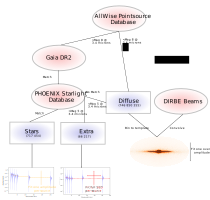
\includegraphics[width=\columnwidth]{figs/diagram/dirbe_diagram.pdf}\\
  \caption{Schematic diagram of the \Cosmoglobe\ DR2 compact object processing pipeline. Red ovals represent input data, and the blue boxes indicate the two classes of sources described in this paper. }
  \label{fig:diagram}
\end{figure}

\subsection{Data model and sampling algorithm}
\label{sec:model}

The objective of this paper is to fit the amplitude of both individual bright stars and the overall diffuse background jointly as part of the global Bayesian \Cosmoglobe\ DR2 analysis framework. The details of this process are discussed by \citet{CG02_01, CG02_02, CG02_07}, and here we only give a brief review of the main points that are directly relevant for starlight modelling.

The basic \Cosmoglobe\ DR2 data model takes the following form,
\begin{align}
	\label{eq:model}
	\dv &=\G\P\B\sum_{c=1}^{n_{\mathrm{comp}}}\M_c\a_c+\s_{\mathrm{zodi}} +
          \s_{\mathrm{static}} + \n_\mathrm{corr} + \n_\mathrm w\\
        &\equiv \s_{\mathrm{tot}} + \n_{\mathrm{w}},
\end{align}
where $\dv$ indicates time-ordered data; $\G$ represents instrumental gain; $\P$ encodes the telescope pointing; $\B$ denotes beam convolution; $\M_c$ is a so-called mixing matrix that defines the relative strength of component $c$ at frequency $\nu$; $\a_c$ is a reference component amplitude; $\s_{\mathrm{zodi}}$ and $\s_{\mathrm{static}}$ are contributions from zodiacal light; and $\n_{\mathrm{corr}}$ and $\n_{\mathrm{w}}$ are correlated and white instrumental noise, respectively. We note that not all parameters are fitted for all channels; see \citet{CG02_01} for details.

As far as this paper is concerned, the key element is $\M_c\a_c$, which defines the astrophysical sky model. In general, this expression includes terms for each relevant physical process, which for the current analysis are thermal dust \citep{CG02_05,CG02_06,CG02_07}, free-free \citep{dickinson2003,planck2014-a12}, CIB (monopoles; \citealp{DIRBE,CG02_03}), and the two starlight populations introduced above. Explicitly, we adopt the following data model for the starlight emission in the following,
\begin{align}
  \M_{\mathrm{stars}}\a_{\mathrm{stars}} &= \sum_{j=1}^{n_{\mathrm{s}}} \M^i_{\mathrm{bright}}\a^i_{\mathrm{bright}} + a_{\mathrm{diff}}\t_{\mathrm{diff}}\\
  &= U^i_{\mathrm{mJy}} \sum_{j=1}^{n_{\mathrm{s}}} \epsilon_j(\nu)\,f_{\mathit{Gaia},j} a_{\mathrm{s},j} + a_{\mathrm{diff}}\t_{\mathrm{diff}}.
  \label{eq:datamodel}
\end{align}
where $U_{\mathrm{mJy}}$ is a unit conversion factor;
$\epsilon_j(\nu)$ is a frequency-dependent extinction factor;
$f_{\mathit{Gaia}}$ is a (bandpass-convolved) SED amplitude per
channel and source; and $a_{\mathrm{s},j}$ is the amplitude per
source, which is the only parameter that is fitted freely per
object. Finally, the second term simply consists of a single overall
diffuse template, $\t_{\mathrm{diff}}$, multiplied with a free
template amplitude per channel. The definition and construction of
each of these factors are described in Sects.~\ref{sec:starmodel} and
\ref{sec:diffusemodel}.

As noted above, the \Cosmoglobe\ DR2 algorithm is a Gibbs sampler, which in practice means that we sample one parameter in Eq.~\ref{eq:model} at a time, while keeping all others temporarily fixed, and then iterate through all parameters. As far as the current paper is concerned, the key steps are therefore to be able to sample from the two following conditional distributions,
\begin{align}
  \a_{\mathrm{bright}} &\leftarrow P(\a_{\mathrm{bright}}| \dv, \G, \M_{\mathrm{dust}}, \a_{\mathrm{dust}}, \s_{\mathrm{zodi}}, \s_{\mathrm{static}}, \n_{\mathrm{corr}}, a_{\mathrm{diff}}) \\
  \a_{\mathrm{diff}} &\leftarrow P(\a_{\mathrm{diff}}|  \dv, \G, \M_{\mathrm{dust}}, \a_{\mathrm{dust}}, \s_{\mathrm{zodi}}, \s_{\mathrm{static}}, \n_{\mathrm{corr}}, a_{\mathrm{bright}}) 
\end{align}
As described by \citet{CG02_01}, in practice this is achieved by 1) subtracting the time-domain correction terms ($\s_{\mathrm{zodi}}$, $\s_{\mathrm{static}}$, and $\n_{\mathrm{corr}}$) from the raw time-ordered data; 2) binning the resulting cleaned data into pixelized maps; 3) subtracting all other astrophysical components except the starlight; and 4) drawing $a_{\mathrm{bright}}$ and $a_{\mathrm{diff}}$ from their  conditional distribution.

To identify the appropriate conditional distribution, we note that a
reduced effective data model may at this point be written in terms of
the following signal-plus-noise residual,
\begin{equation}
  r = \M_{\mathrm{stars}}\a_{\mathrm{stars}} + \n_{\mathrm{w}}. 
\end{equation}
Since $\n_{\mathrm{w}}$ denotes white Gaussian noise, and $\M$ is a fixed matrix, this is a perfectly linear data model in $\a$, and the appropriate conditional probability distributions, $P(a_{\mathrm{bright}}|\dv,\ldots)$ and $P(a_{\mathrm{diff}}|\dv,\ldots)$, are both Gaussian. The appropriate sampling equation is therefore \citep[see, e.g., Appendix~1 in][]{bp01}
\begin{equation}
  \a_{i} = (\M_i^T \N^{-1} \M_i)^{-1} \M_i(\r-\M_j\a_j),
\end{equation}
where $\{i,j\}$ now denote respectively bright or diffuse sources in a given Gibbs step, and then the reverse combination in the next Gibbs step. This algorithm is then iterated until convergence, and interspersed with similar Gibbs steps for all other free parameters in Eq.~\ref{eq:model}.


\subsection{Bright stars}
\label{sec:starmodel}

To complete the above algorithm, we need to specify $\M$, $\t$, and $\n_{\mathrm{s}}$, and we start by defining the catalog of bright stars. The first step in this procedure is to threshold the AllWise point source catalog \citep{wiseCat} at magnitude 7 in the W1 band. This results in a set of \textbf{N} unique objects. Unfortunately, many of these are located spatially very close to each other, and given the wide DIRBE beam this results in strong degeneracies in the fitted parameters of near-by objects. Furthermore, as described above, the computational engine of the current analysis framework is a Gibbs sampler, which is known to have a long correlation length for strongly correlated parameters \citep{geman:1984}. For this reason, we divide the set of bright objects into three separate sampling groups, within each of which no two objects are closer than a given distance. Specifically, each set is constructed by including the brightest remaining object, but only if it is further away from any already included source than 5'. 

For each star in these sampling groups we extract estimates of the effective temperature, $T_{\mathrm{eff}}$, the gravitational acceleration, $\log g$, and the metallicity, $[M/H]$, from the \GAIA\ DR2 database \citep{gaiaCat}, and use those to identify a best-fit spectral energy density (SED) from the PHOENIX starlight database \citep{Husser_2013}. The distributions of these parameters for the selected stars are shown in Fig.~\ref{fig:gaiacat}. Unfortunately, the PHOENIX catalog lacks information for $T_{\mathrm{eff}} > 12000$\,K, and these we use the closest match; this accounts for 1.1\,\% of all bright WISE objects. In principle, this may lead to a bias in the SEDs for the hottest stars, but this effect is at least partially mitigated by the fact that we fit the overall amplitude of each star freely in the following analysis. 

\begin{figure}
  \includegraphics[width=0.96\columnwidth]{figs/gaia/t_eff.pdf}
  \includegraphics[width=0.96\columnwidth]{figs/gaia/logg.pdf}\\
  \includegraphics[width=0.96\columnwidth]{figs/gaia/metalicity.pdf}\\
  \caption{Histograms of the three star parameters (effective temperature, gravitational acceleration, and metallicity) that are used by the PHOENIX database to determine the star SEDs, for the 424\,829 stars used in this analysis.}
  \label{fig:gaiacat}
\end{figure}

The relationship between the physical stellar parameters and the resulting star SEDs is illustrated in Fig.~\ref{fig:catalogueSEDs}. The black curves in each panel shows the SED for a typical star with $T_{\mathrm{eff}}= 6000$\,K, $\log g = 3$ and $[M/H]= 0.0$, while the colored curves shows the SEDs resulting by changing one parameter at a time. As expected, the effective temperature has the biggest effect on the overall SED, especially when averaged over wide observing bands like those of DIRBE, while the other two parameters only have a relatively mild impact. This is further illustrated in Fig.~\ref{fig:logg_ratio}, which shows the ratio between two spectra with $\log g = 5$ and 0, and with the DIRBE channel center frequencies indicated as vertical dashed lines. Here we see that neglecting $\log g$ would lead to a 1-2\,\% relative bias between the 1.25 and 3.5\,$\mu$m channels.

\begin{figure}
\includegraphics[width=0.85\columnwidth]{figs/gaia/star_SED_Teff.pdf}
\includegraphics[width=0.85\columnwidth]{figs/gaia/star_SED_logg.pdf}
\includegraphics[width=0.85\columnwidth]{figs/gaia/star_SED_MH.pdf}
  \caption{Comparison of PHOENIX spectra for different parameter compbinations. In each panel the black curve shows a reference star spectrum with $T_{\mathrm{eff}}= 6000$K, $\log g = 3.0$ and $[M/H]= 0.0$. The colored curve shows, from top to bottom, the resulting spectra when setting $T_\mathrm{eff}=10\,000\,\mathrm{K}$, $\log g = 5.0$, and $[M/H]= -2.0$. The spectra shown in the middle panel have been smoothed to highlight the broad features that are mostly relevant for the current analysis.}
  \label{fig:catalogueSEDs}
\end{figure}

\begin{figure}
\includegraphics[width=\columnwidth]{figs/gaia/star_SED_logg_ratio_v2.pdf}
\caption{Ratio between the PHOENIX spectra shown in the middle panel of Fig.~\ref{fig:catalogueSEDs}, corresponding to $E(\log g = 5)/E(\log g  = 3)$. The vertical dashed lines indicate the positions of the six shortest wavelength DIRBE channels.}
  \label{fig:logg_ratio}
\end{figure}



\subsubsection{The PHOENIX Database}
\label{sec:phoenix}

To build an optimal SED model for each stellar source given the parameters retrieved from \GAIA, we perform a few post-processing steps for the spectra provided by the PHOENIX database. First, PHOENIX provides spectra in finite resolution bins, as summarized in Table~\ref{tab:phoenix}, whereas the parameters estimated from the \GAIA\ data have arbitrary precision. Instead of simply selecting the closest spectrum to each star, we compute a linear combination of the nearest six spectra, weighted by distance from the measured value, as given by 
\begin{align}
s &= \frac{1}{3}\bigg[\frac{s_{T-} (T_{+} - T) + s_{T+} (T - T_{-})}{T_{+} - T_{-}} \nonumber \\ 
&+ \frac{s_{g-} (g_{+} - g) + s_{g+} (g - g_{-})}{g_{+} - g_{-}} \nonumber \\
&+ \frac{s_{M-} (M_{+} - M) + s_{M+} (M - M_{-})}{M_{+} - M_{-}}\bigg].
\label{eq:starspec}
\end{align}
Here, $s$ represents a single spectrum, and we have used $T$, $g$ and $M$ as short forms for $T_{\mathrm{eff}}$, $\log g$ and $[M/H]$. The subscripts + and $-$ correspond to the closest reference value above and below the measured value (for example, 0.0 and 0.5 if $\log g=$0.315). 

\begin{figure}
  \centering
  \includegraphics[width=\columnwidth]{figs/extinction/dirbe_extinction_1a.pdf}\\
  \caption{The full-sky extinction template used in this analysis, evaluated in the DIRBE 01 band at $1.25\mu$m.}
  \label{fig:ext_template}
\end{figure}


A second complicating factor is that the updated release of the catalogue\footnote{\href{https://www.astro.uni-jena.de/Users/theory/for2285-phoenix/grid.php}{\texttt{https://www.astro.uni-jena.de/Users/theory/\newline for2285-phoenix/grid.php}}} contains only a subset of the files in the original catalogue, although they are believed to be more accurate. For stars the extended parameter range, most importantly those with $\log g<$3.0, we therefore calculate spectra using the older files. 

Unfortunately, the older files are only defined up to $\lambda=5.5\mu$m, compared to the newer files, which extend to $\lambda=50\mu$m. Amplitude estimates for these stars in the $12\mu$m and $25\mu$m bands must therefore be determined by, first, computing the spectra with the old PHOENIX files and the new PHOENIX files, using the closest endpoint ($\log g$=3.0 in the most common case). Then, we compute the ratio between the amplitudes of the $3.5\mu$m and $4.9\mu$m channels, and exploit the obseration in Fig.~\ref{fig:logg_ratio} that the spectrum ratio is nearly constant above 4.9\,$\mu$m to extrapolate into longer wavelenghts.

\begin{table}
    \centering
    \newcolumntype{C}{ @{}>{${}}r<{{}$}@{} }
    \begin{tabular}{l c c c c c }
    \hline
    \hline
     Param & Step Size & \multicolumn{2}{c}{Old} & \multicolumn{2}{c}{Updated}\\ 
     & & Min & Max & Min & Max\\
    \hline
    \hline
    $T_{\mathrm{eff}}$ (K) & 50-100K & 2300K & 12000K & 3000K & 11900K\\
    $\log g$ & 0.5 & 0.0 & 6.0 & 3.0 & 5.0 \\
    $[M/H]$ & 0.5 & -4.0 & 1.0 & -2.0 & 1.0 \\
     \hline
    \end{tabular}
    \caption{Parameters of spectra provided by the PHONEIX starlight database, both for the original and updated spectra.}
    \label{tab:phoenix}
\end{table}

\begin{figure}
  \centering
  \includegraphics[width=\columnwidth]{figs/diffuseTemplate/diffuse_template.pdf}\\
  \caption{The unsmoothed template of diffuse star emission evaluated in the DIRBE 01 band, plotted on a log scale.}
  \label{fig:diffuse}
\end{figure}

\subsubsection{Binary Stars}

About 25\% of entries stronger than 12 mag were found to be binary stars in the \Gaia\ database, and for many of these individual physical parameters are provided for each star separately. When modelling these in DIRBE, which has a low angular resolution, the two contributions must be averaged into one effective SED. For these, we first calculate the spectrum of each component according to Eq.~\ref{eq:starspec}. Since the flux values are given per unit of area, we then weigh the two spectra according to the estimated area of the corresponding star, so that the total flux estimated from the binary system reads
\begin{equation}
    s_{\mathrm{b}} = \frac{s_1 r_1^2+ s_2 r_2^2}{r_1^2 + r_2^2},
\end{equation}
where $s_{1, 2}$ and $r_{1, 2}$ denotes the flux and radius of the respective star in the binary system. The radii are not given explicitly in the \GAIA\ catalogue, so we therefore estimate their radius as \citep{kuiper_1938}
\begin{equation}
r = \exp\left(\frac{3.5\cdot 4}{5(3.5 \log(T_{\mathrm{eff}}) - \log(g))}\right ).
\end{equation}

\begin{figure*}
  \centering
  \includegraphics[width=0.45\textwidth]{figs/starmaps/all_stars_mean_01.pdf}
  \includegraphics[width=0.45\textwidth]{figs/starmaps/all_stars_mean_02.pdf} \\
  \includegraphics[width=0.45\textwidth]{figs/starmaps/all_stars_mean_03.pdf}
  \includegraphics[width=0.45\textwidth]{figs/starmaps/all_stars_mean_04.pdf} \\
  \includegraphics[width=0.45\textwidth]{figs/starmaps/all_stars_mean_05.pdf}
  \includegraphics[width=0.45\textwidth]{figs/starmaps/all_stars_mean_06.pdf} \\
  \caption{Mean star maps from the Cosmoglobe DR2 release for the first six DIRBE bands. }
  \label{fig:starsT}
\end{figure*}


\subsubsection{Extinction}
\label{sec:extinction_model}

At the highest frequencies, dust extinction becomes important, particularly in the Galactic plane. In this paper, we model this effect by $\epsilon(\nu)$, which we defined as the ratio between the observed and the intrinsic flux from a given star, i.e., comparing the flux with and without dust extinction. We construct a simplified model for this based on the work by \cite{ext_model} and \cite{fitzpatric_19}. Specifically, we implement their 47-parameter model that extends from UV to infrared frequencies,\footnote{Note that we believe there is a typo in \cite{ext_model}, which has added an additional negative sign on their value of $b_{IR}\ \alpha_{1}$, and the correct value should be 1.06099}, which provides a general sky-averaged estimate of the dust extinction, $\epsilon(\nu)$. 

To account for spatial varations, we combine this averaged spectral behaviour with the $E(B-V)$ map from the \Planck\ 2013 dataset \citep{planck_extinc_2013}, starting from Eq.~1 of \cite{ext_model}:
\begin{equation}
\frac{A(\lambda)}{A(V)} = a(\lambda) + b(\lambda)\left[ \frac{1}{R(V)} - \frac{1}{3.1}\right].
\end{equation}
Here, $\lambda$ is wavelength, $A$ is the absolute extinction, and $a$ and $b$ are the model coefficients listed by \citet{fitzpatric_19}. Finally, $R(V)$ is given by
\begin{equation}
R(V) = \frac{A(V)}{E(B-V)},
\end{equation}
and therefore denotes the ratio of absolute to selective extinction in the V-band. Substituting this relationship into the above equation, and using the full sky average case of $R(V) =3.1$ \citep{fullsky_ext}, allows us to omit the $b$ terms, and we simply obtain
\begin{equation}
A(\lambda) = 3.1\, E(B-V) a(\lambda).
\end{equation}
Finally, we convert from magnitudes to the linear $\epsilon(\nu)$ scaling factor to obtain
\begin{equation}
\epsilon(\lambda) = \frac{F_{\mathrm{ext}}}{F_{\mathrm{raw}}} = e^{-\frac{3.1}{2.5} E(B-V) a(\lambda)}.
\end{equation}

\begin{figure*}
  \includegraphics[width=0.95\textwidth]{figs/zoom/combined_zoom.pdf}\\
  \vspace{-8pt}
  \hspace{1.2in}
  \includegraphics[scale=0.7]{figs/zoom/cbar1.pdf}
  \hspace{0.95in}
  \includegraphics[scale=0.7]{figs/zoom/cbar2.pdf}
  \hspace{0.15in}
  \includegraphics[scale=0.7]{figs/zoom/cbar4_chisq.pdf}
  \caption{Zoom-ins on a subregion of the sky centred at $(20^\mathrm{o},70^\mathrm{o})$. The third column shows the (data-minus-model) difference between the two, and the final column shows the overall chisq of the component separation fit.}
  \label{fig:zooms}
\end{figure*}

The resulting spatial extinction template, evaluated for the 1.25$\mu$m band, can be seen in Fig.~\ref{fig:ext_template}. The majority of the extinction is occurring in the Galactic plane, but additional contributions can be seen tracing dust structures at high galactic latitudes. The template scales according to the relations shown in Fig.~7 of \cite{ext_model}, and is applied to the stars component as described in Eq.~\ref{eq:datamodel}.

\begin{figure*}
  \centering
  \includegraphics[width=0.34\textwidth]{figs/mixing/trace_1352704.pdf}
  \includegraphics[width=0.31\textwidth]{figs/mixing/trace_2429499.pdf}
  \includegraphics[width=0.31\textwidth]{figs/mixing/trace_3121308.pdf}\\
  \caption{Trace plots of the total star amplitude in both chains for three pixels in different regions of the sky (low latitudes, the LMC and high latitudes) in the DIRBE 1.25\,$\mu$m band. The dashed vertical line indicates the end of the burn in period, and samples after that are included in our final sample set.}
  \label{fig:amptrace}
\end{figure*}

\begin{figure}
  \centering
  \includegraphics[width=\linewidth]{figs/correlation/covmatrix.pdf}
  \caption{Correlation plot showing a selection of parameters relevant for star modelling. From top to bottom: the monopoles for DIRBE channels between 1.25 and 4.9\,$\mu$m; $N_{0}$ and albedoes for bands 1-3 which are the full sky ZL parameters; full-sky dust amplitudes for the nearby and hot dust components; the amplitudes of three randomly selected stars and the diffuse template amplitude for bands 1-4.}
  \label{fig:corr}
\end{figure}

We conclude this section by noting that the extinction model used here is indeed simplified, as it does not take into account the actual 3D position of each star, but rather assume the \Planck\ $E(B-V)$ map to be valid for any position along a given line of sight. Because most of the dust signal observed by \Planck\ originates from dust grains closer than a few hundred parsecs from the Sun, this approximation is likely to be significantly better at high Galactic latitudes than for positions near the Galactic plane. Still, because of this approximation, we exclude the 1.25\,$\mu$m channel, for which extinction is far more important than at longer wavelengths, when estimating $\a_{\mathrm{bright}}$.

\subsection{Diffuse Star Emission}
\label{sec:diffusemodel}

After modelling the brightest sources using the method described above, we are left with a diffuse background of stars that are too dim to be individually resolved, but that in aggregate form a significant contribution to the total star signal at these wavelengths and so must be accounted for. We model this diffuse background using a single full-sky template, generated from the WISE W1 data at 3.4$\mu$m. We take the full AllWISE point source catalog, and select all sources with a valid W1 magnitude that are not already included in the bright point source model. To account for pixelization effect, we create this template at high resolution (HEALpix $N_{\mathrm{side}}=2048$), co-adding over all sources with their appropriate SED and beam profiles, and then downgrade to $N_{\mathrm{side}}=512$ to match the resolution of the observed DIRBE maps. The resulting map shown in Fig.~\ref{fig:diffuse}. This template is then included in the full sky model in Eq.~\ref{eq:model}, with an amplitude fit separately for each channel. 


\section{Astrophysical results}
\label{sec:results}

The model described in the previous section is then included in a full sky model, which includes galactic dust, zodical light and other components. A model of the DIRBE instrument is used to estimate other data artifacts, the most prominent of which was a sun-stationary signal of unknown origins. Following our previous work withing the Cosmoglobe framework \citep{bp01, watts2023_dr1}, we implement this model within the \texttt{commander3} codebase \citep{bp03}, which is our Bayesian end-to-end analysis pipeline. The full posterior of all our model parameters was then sampled using Gibbs sampling, exploring the full space around the maximum likelihood values of each parameter. We computed a total of 1090 unique samples spread over 5 independent chains after discarding our 25 samples of burn-in data, which gave robust sample sizes for the results described here. 

In this paper, we present just the results of the star models described in section \ref{sec:models}, but we direct interested readers to the companion papers in the larger data release. More details on the overall sampling approach can be found in \citet{CG02_01}. The other components of the sky model are described in \citet{CG02_02}, \citet{CG02_05}, \citet{CG02_06} and \citet{CG02_07} and our limits on the CIB monopole derived from this work are presented in \citet{CG02_03}. 


\subsection{Maps}

In Figure \ref{fig:starsT} we show the mean star maps for the full pipeline run in all six DIRBE bands where they are modelled. Here, the maps show the sum of the star component and the diffuse background, which accounts for the  majority of the point source emission over the full sky. As expected, the emission is concentrated in the galactic plane, but there is also an important contribution from high latitude stars.

In Figure \ref{fig:zooms} we show zoom ins of a 20$^\mathrm{o}$ patch of sky centered at (lon, lat)= $20^\mathrm{o}, 70^\mathrm{o}$, plotting the DIRBE sky map in each band for the four highest frequency bands where the stars are most significant. In the second column, we show the total star model for the same region, then the resulting residual, and finally the overall chisq of the fit. The residuals contain a variety of mis-modeled point sources.

We can identify three types of point source residuals in this third column, although there are a large number of sources with residuals that are subdominant to the background noise level and so can be considered to be well modelled. Some of the point sources clearly show the imprints of spectral complexity, where the residual signature is blue in some bands and red in some others, which implies that our knowledge of the spectra is imperfect and a single overall amplitude fit will always be insufficient to model that source. The second class of residuals appear to be ring shapes, where the center of the point source is well modelled, but we oversubtract emission around the edges. This could be caused by our simplistic modelling of the DIRBE beams, which relies on the scanning strategy to symmeterize the otherwise square beam profile of the DIRBE instrument.

Other point source residuals are more complex, and look to be superpositions of multiple sources in the same region. These residuals could possibly be reduced by pruning point sources from the model that are too close to one another, or potentially by improving our models of the brightest sources. No attempt to do so was made in this work, as these residuals were only a small fraction of the total sky, and can be handled by masking using the chisq, which clearly shows these regions to be poorly modelled.



In Figure \ref{fig:amptrace}, we show the total amplitude of the stars in three pixels in different regions in the sky (low Galactic latitudes, the Large Magellanic Cloud and high Galactic latitudes) as a function of iteration, for all five of our  independent sampling chains. The first 25 samples in each chain are discarded as burn in, and the remaining samples (1090 in total) form the samples included our analysis. We see good mixing of the total amplitudes in the top row, although examining the individual components we do note that the full sky diffuse template mixes slower than the individual bright stars.


Figure \ref{fig:corr} shows the correlation matrix, computed between each parameter over all 1090 samples. In this case, we include a sample of star parameters, as well as some other parameters where we suspect degeneracies may occur. We see correlations between the monopoles of the 01, 02 and 03 bands, as well as between some of the zodiacal light parameters, as has been studied in \citep{CG02_01, CG02_02}, but low correlation between these and the star model parameters, implying that they are relatively independent. We do not see much cross correlation between the star parameters and other parameters in the global chain, with the exception of some of the individual star parameters and the dust amplitudes, which seem to be anti-correlated. This implies that overall the star parameters are well mixed and are not degenerate with other full sky parameters in the run.

\subsection{Spectral Energy Densities}

In addition to the amplitude maps at each frequency, we can also examine the spectra energy densities (SEDs) of the sources within our model. Figure \ref{fig:starSEDs} shows the median SED model for all 424\ 829 star sources in our catalogue, as well as the SED for the diffuse template component, both normalized to the same amplitude in band 1. These follow a similar overall shape, although the diffuse stars fall off faster than the bright stars as we go to increasing wavelengths, perhaps due to selection effects between the two sets.

\begin{figure}
  \includegraphics[width=\columnwidth]{figs/starseds/star_seds.pdf}
  \caption{Star emission as a function of wavelength. The orange line is the median of all the individual stars fit in the model, with a variance computed across all samples that is too small to see on this plot. The red curve is the mean of the diffuse template SED fit to the data, with the error bars showing the variance across the chain.}
  \label{fig:starSEDs}
\end{figure}

\subsection{Extinction}

We also investigate our model of extinction, to determine how it compares to other estimates. Figure \ref{fig:extinction} shows the mean star emission as a function of galactic latitude, zoomed in on the central region. The three curves are the DIRBE Faint Source Model, used in the legacy analysis \citep{dirbeFaint}, as well as our diffuse star model and the Cosmoglobe total star emission estimate. Overplotted as dashed lines are linear fits to the data between 5 and 1 degrees, which, when extrapolated to the galactic center region, give some approximation of the star signal in the absence of extinction. By comparing the peak amplitude of the fit to that of the models, we can get an approximate amplitude of extinction in the galactic center, which we can compare to the estimate from our extinction template (black line) which predicts about a 50\% extinction. We see that the FSM estimates a ration of around 0.75 in the central region of the galaxy, and our model produces something in the range of 0.9, which is mostly likely an underestimate of the total extinction on the sky. Because our extinction coefficient is applied only to the bright sources, the diffuse template contribution (which is about three quarters of the total power) at 1.25 $\mu m$ is too high in the galactic center, leading to an overall underestimate of the extinction. Future work should be done to improve on this limitation of our model.

 %previous estimates such as \cite{extinction} estimate it at 70\% at 1 $\mu$m and 94\% at 3.4 $\mu$m.

\begin{figure}
\includegraphics[width=\columnwidth]{figs/diffuseTemplate/extinction.pdf}
  \caption{Profiles of the DIRBE Faint Star Model (FSM) and Cosmoglobe star model as a function of galactic latitude. A linear extrapolation is overplotted in the core region from -5 to 5 degrees galactic latitude, but excluding the galactic center from -1 to 1 degree. The theoretical value central value from this fit is compared to the measured values in the central bins to give estimates of the dust extinction in the galactic center for both cases.}
  \label{fig:extinction}
\end{figure}

\section{Comparison to other Analyses}
\label{sec:consistency}

\begin{table*}
    \centering
    \newcolumntype{C}{ @{}>{${}}r<{{}$}@{} }
    \begin{tabular}{l c c c c c c c c c}
    \hline
    \hline
     Patch & $l$ & $b$ & $r$ & \multicolumn{2}{c}{Bright Stars} & \multicolumn{2}{c}{Diffuse Stars} & \multicolumn{2}{c}{Sum}\\ 
     & ($^{\circ}$) & ($^{\circ}$) & ($^{\circ}$) & \multicolumn{2}{c}{(kJy/sr)} & \multicolumn{2}{c}{(kJy/sr)} & \multicolumn{2}{c}{(kJy/sr)}\\
          &  & & & \cite{DIRBE2mass} & CG & \cite{DIRBE2mass} & CG  & \cite{DIRBE2mass} & CG\\
    \hline
    \hline
    \multicolumn{10}{c}{1.25$\mu$m}\\
    \hline
     1 \rule{0pt}{2ex} & 127.3 & 63.8 & 1.5 & 31.56 & 13.0 & 3.08 & 38.3 & 34.64 & 51.4\\
     2 & 107.7 & 57.7 & 2.0 & 42.72 & 18.8 & 3.62 & 44.5 & 45.34 & 63.3\\
     3 & 157.0 & -82.7 & 2.0 & 40.89 & 20.0 & 2.94 & 40.0 & 43.83 & 60.1\\
     4 & 257.8 & -59.4 & 1.9 & 51.88 & 28.6 & 3.92 & 45.3 & 55.8 & 73.9\\
     \hline
     \hline
     \multicolumn{10}{c}{2.2$\mu$m}\\
     \hline
     1 \rule{0pt}{2ex} & 127.3 & 63.8  & 1.5 & 20.79 & 9.0 & 1.58 & 25.7 & 22.37 & 34.7\\
     2 & 107.7 & 57.7 & 2.0 & 28.99 & 13.6 & 1.87 & 29.9 & 30.86 & 43.4\\
     3 & 157.0 & -82.7 & 2.0 & 28.62 & 15.1 & 1.50 & 26.9 & 30.12 & 42.0\\
     4 & 257.8 & -59.4 & 1.9 & 36.16 & 21.6 & 2.03 & 30.4 & 38.19 & 52.0\\
     \hline
    \end{tabular}
    \caption{Comparison of component intensities in patches from \cite{DIRBE2mass} and Cosmoglobe (CG) at 1.25 and 2.2 $\mu$m. The galactic longitude and latitude of the region center are given by $l$ and $b$, and $r$ is the radius of the field. The definitions of bright and diffuse sources differ between analyses, but the sum of the two allow reasonable comparison.}
    \label{tab:2mass}
\end{table*}


\subsection{DIRBE FSM}

The original DIRBE analysis team \citep{dirbeFaint} also removed point sources from their measurement of the CIB emission, but followed a different approach. Instead of modelling the bright sources, the original analysis simply masked pixels brighter than a threshold (15 Jy in band 01), which resulted in cutting almost 35 \% of the sky at 1.25 $\mu$m. For the diffuse sources, they build a model (the ``faint source model'' or FSM) using the mechanism of \cite{wainscoat}, which integrates a model of source counts over the full sky, including models of galactic morphology, 87 discrete source types and the contribution from dust extinction. The results of this model in the DIRBE 01 band are shown in Figure \ref{fig:DIRBEfaint}, as well a comparison of the two models. 

The top two panels of Figure \ref{fig:DIRBEfaint} shows our diffuse template and the FSM, converted from QuadCube to HEALpix and plotted at nside=256. The third image shows the difference between these two templates of diffuse star emission, which clearly shows a difference in the galactic center, driven by extinction as discussed above. 

\begin{figure}
\includegraphics[width=0.9\columnwidth]{figs/diffuseTemplate/diffuse_mean.pdf}  \vspace{-4pt}\\
  \includegraphics[width=0.9\columnwidth]{figs/diffuseTemplate/dirbe_template.pdf}\\
  \includegraphics[width=0.9\columnwidth]{figs/diffuseTemplate/diffuse_diff.pdf}\\
  %\includegraphics[width=0.9\columnwidth]{figs/diffuseTemplate/band_01_map.pdf}\\
  \includegraphics[width=0.9\columnwidth]{figs/diffuseTemplate/band01_res.pdf}\\
  \caption{The Commander diffuse star template (Top). Next: The DIRBE faint star model at 1.25 $\mu$m retrieved from LAMBDA and converted from QuadCube to healpix and the difference between that model and the diffuse template (position 3). The bottom panel shows the DIRBE 01 residual from the Commander run, indicating that our star model is slightly overestimating signal in the galactic plane, likely due to underestimated extinction. At high latitudes, the two models show good morphological agreement.}
  \label{fig:DIRBEfaint}
\end{figure}

\begin{figure*}
  \centering
  \includegraphics[width=\textwidth]{figs/sed/cg_spec_DR2_en.pdf}
  \caption{Components of the infrared temperature sky from 1$\mu$m to 1m wavelengths. The approximate contribution from stars is shown in yellow, and the observing bands from various experiments are indicated by the vertical lines. }
  \label{fig:sed}
\end{figure*}


This difference shows that our model based on the integrated AllWISE point source catalogue predicts more star emission in the galactic plane than the DIRBE FSM in the inner part of the plane where dust extinction is dominant. However, when we look at the $1.25 \mu m$ residual map in the bottom, it is clear that the model is actually underpredicting signal in this region, so more extinction is disfavoured by the data in this run.

In the galactic bulge, our model predicts less emission than the FSM, which, when we look at the bottom panel of fig. \ref{fig:DIRBEfaint}, seems to be a better fit to the data. The blue residuals in the galactic center show that the model overpredicts emission in general in the bulge, so  increasing the emission to the level that the FSM predicts would be a worse fit in this region. 

\subsection{DIRBE and 2MASS}

After the official DIRBE analysis, \cite{DIRBE2mass}, following \cite{gorjian} used the 2MASS catalogue to remove star emissions from DIRBE and find an improved upper limit on the CIB monopole, but were ultimately unable to claim a detection due to the zodiacal light contamination that they could not correct for. Their analysis looked at four dark patches of the sky and used 2MASS to estimate the contribution of both bright (K band magnitude > 14) and faint sources to the total signal in each patch, which we can compare with the Cosmoglobe estimates in those same regions, as shown in Table \ref{tab:2mass}.


Differences in star classification between our analysis and \cite{DIRBE2mass} make it challenging to directly compare our amplitude estimates, but the sum of the bright and diffuse sources can still be compared. The Cosmoglobe analysis predicts about 40\% more total star emission, depending on the field and the frequency, which is probably due to having a much deeper and more complete star catalogue than 2MASS. By successfully modelling and removing more star emission, we are able to improve upon their limits on the CIB, as discussed in \cite{CG02_03}. 

\section{Conclusions}
\label{sec:conclusions}

Stars are a critical component of the infrared sky, which must be correctly modelled in order to avoid contaminating other components. This paper produced a complete model of the star emission in the infrared, which was able to account for the vast majority of the star signal. Using data from \Gaia\ and \WISE\, we constructed models of 424\ 829 individual point sources as well as a diffuse background of the remaining 710\ 825\ 587 sources, which was able to model 91\% of the observed DIRBE flux density at 2.2$\mu$m, dropping to 1\% at 25$\mu$m.

Figure \ref{fig:sed} shows the full sky average star SED derived from this work, plotted with the other sky signals as a function of frequency and wavelength, from the radio all the way to the infrared. The Cosmoglobe DR2 release, which this paper forms part of, is the first time a unified model of the sky has been shown to successfully describe all these frequencies, and the star model presented here is an integral part of this work.

The star model showed robust mixing, and was able to fully describe the summed star emission in an effective manner. Our model was able to characterize and remove more star emission than previous works, which consequently was able to produce lower residuals and better constraints on the CIB monopoles, as discussed in the companion paper \citet{CG02_03}. This work is a part of the first full-sky estimate of the monopole which agrees with theory in the $1 \mu m$ region, and properly including this deep background of diffuse stars was the critical component to this effort. Previous iterations of our pipeline produced estimates that were more in line with existing limits, and after some investigation, we discovered a bug in our diffuse template implementation which had omitted the dimmest objects. Properly accounting for those sources was what allowed us to achieve the limits shown in \citet{CG02_03}.

\subsection{Future Work}
The star model could be improved by updating the dust extinction model. While this paper incorporates a first-order extinction correction, it is based on a full-sky template taken from the Planck estimate of extinction of CMB photons. To get accurate numbers for stars that are embedded in the Galaxy, we would need to incorporate 3-D position information from \gaia\ to determine the line-of-sight extinction to each source. Constructing a 3-D model of all the stars and gas in our Galaxy is beyond the scope of this paper, but could be an intriguing area of future research combining  these large modern datasets. 

Another place within the model where there is room for more work is in the treatment of the beams. Instead of assuming spherically symmetrized beams, we could properly treat the unique square shape of the DIRBE response function, using techniques like deconvolution mapmaking \citep{artdeco}. This could potentially resolve some of the ``ring'' residuals around bright sources.

We could also improve our handling of the brightest stars, determining more accurate SEDs for those with $T_{\mathrm{eff}}>12000$K. This may help reduce the residuals around the brightest sources, and, combined with pruning the bright sources with 0 amplitudes could reduce the overall residual levels around these bright sources. A more complete catalogue of star SEDs with higher resolution and expanded parameter ranges in the infrared would also improve the modelling of the individual sources, leading to lower residuals and fewer chi-squared cuts.

Finally, including additional high frequency data directly in the the full run would be an important next step for this work, and will be the subject of future exploration in the collaboration. WISE is a major candidate experiment here, but also AKARI \citep{akari}, SPHEREx \citep{Crill_2020} and \IRAS\ \citep{neugebauer:1984} would be important complements to the work performed here. Incorporating these data directly should give enough extra information to constrain the star SEDs directly instead of having to extrapolate them from other regimes. The \Cosmoglobe\ project is already in the process of working with some of these data, and so improved results in the infrared regime should be forthcoming.

\begin{acknowledgements}
MG would like to thank Prof. Alberto Dominguez for useful conversations that led to improvements in the star modelling and better limits on the CIB monopoles at 1.25 $\mu$m.
 The current work has received funding from the European
  Union’s Horizon 2020 research and innovation programme under grant
  agreement numbers 819478 (ERC; \textsc{Cosmoglobe}) and 772253 (ERC;
  \textsc{bits2cosmology}). Some of the results in this paper have been derived using the HEALPix \citep{healpix} package.
  We acknowledge the use of the Legacy Archive for Microwave Background Data
  Analysis (LAMBDA), part of the High Energy Astrophysics Science Archive Center
  (HEASARC). HEASARC/LAMBDA is a service of the Astrophysics Science Division at
  the NASA Goddard Space Flight Center.  
  
   This publication makes use of data products from the Wide-field Infrared Survey Explorer, which is a joint project of the University of California, Los Angeles, and the Jet Propulsion Laboratory/California Institute of Technology, and NEOWISE, which is a project of the Jet Propulsion Laboratory/California Institute of Technology. WISE and NEOWISE are funded by the National Aeronautics and Space Administration.
   
   This work has made use of data from the European Space Agency (ESA) mission
{\it Gaia} (\url{https://www.cosmos.esa.int/gaia}), processed by the {\it Gaia}
Data Processing and Analysis Consortium (DPAC,
\url{https://www.cosmos.esa.int/web/gaia/dpac/consortium}). Funding for the DPAC
has been provided by national institutions, in particular the institutions
participating in the {\it Gaia} Multilateral Agreement.

This paper and related research have been conducted during and with the support of the Italian national inter-university PhD programme in Space Science and Technology. Work on this article was produced while attending the PhD program in PhD in Space Science and Technology at the University of Trento, Cycle XXXIX, with the support of a scholarship financed by the Ministerial Decree no. 118 of 2nd March 2023, based on the NRRP - funded by the European Union - NextGenerationEU - Mission 4 "Education and Research", Component 1 "Enhancement of the offer of educational services: from nurseries to universities” - Investment 4.1 “Extension of the number of research doctorates and innovative doctorates for public administration and cultural heritage” - CUP E66E23000110001.
\end{acknowledgements}


%-------------------------------------------------------------
%                                       Table with references 
%-------------------------------------------------------------
%

\bibliographystyle{aa}
\bibliography{references, ../../common/CG_bibliography,../../common/Planck_bib}
\end{document}
%%%% End of aa.dem


